\documentclass{article}
\usepackage{graphicx}
\graphicspath{./assets/}

\title{IB HL Physics - Gravitation}
\author{Zitang Ren}
\begin{document}

\maketitle

\section{Newton's Law of Universal Gravitation and Gravitational Force}
Newton was the first to recognise that the speed of a falling object on Earth is the same as the force that governs the motion of the moon.
His universal law states that: \textbf{Every particle of matter in the universe attracts every other particle with a gravitational force that is directly proportional to the product of the masses of the particles and inversely proportional to the square of the distance between them.}
\\
\\In equation form, this is:
\begin{equation}
    F=\frac{GMm}{r^2}
\end{equation}
\\Where: $F$ is the magnitude of force between the particles, $G$ is the universal gravitational constant, $M$ is the mass of one particle, $m$ is the mass of the other particle, and $r$ is the distance between the particles.
\begin{center}
    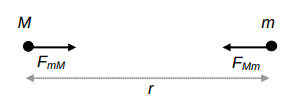
\includegraphics[scale=0.6]{assets/arrowForce.png}
\end{center}\leavevmode
The gravitational force exerted by a spherical mass on a particle is the same as if the mass of the sphere were concentrated at its centre.
\begin{center}
    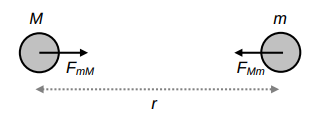
\includegraphics[scale=0.6]{assets/sphereForce.png}
\end{center}\leavevmode

\pagebreak
\subsection*{Worked Example 1}
The mass of the Earth is 81 times that of the moon and the distance from the center of the Earth to that of the moon is about $3.8\times10^5$km.
Calculate the distance from the center of the Earth where the resultant gravitational force becomes zero when a spacecraft is launched from the Earth to the moon.
\begin{center}
    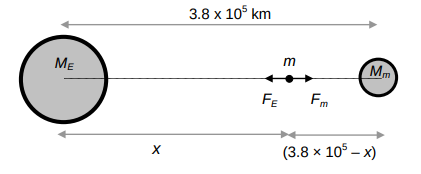
\includegraphics[scale=0.6]{assets/sec1ex1.png}
\end{center}\leavevmode
\textbf{Solution}
\\Since the gravitational foce of the Earth on the spacecraft is acting opposite to that of the moon, at distance $x$ from the Earth,
the gravitational force of the Earth will be equal to that of the moon:
\\
\begin{equation}
    \frac{GM_{Earth}m}{x^2}=\frac{GM_{moon}m}{(3.8\times10^5-x)^2}
\end{equation}
\begin{equation}
    \frac{x^2}{(3.8\times10^5-x^2)}=\frac{M_{Earth}}{M_{moon}}=\frac{81}{1}
\end{equation}
\\
\begin{equation}
    10x=3.42\times10^6
\end{equation}
\\
\begin{equation}
    x=3.4\times10^5
\end{equation}
\pagebreak
\section{Gravitational Field}
A field of force is a region of space where a force is found to act on a body placed in it. \textbf{A gravitational field is a region of space in which a mass experiences a force due to the presence of another mass.}
A large mass $M$ will produce a gravitational field in the space around it. A small mass $m$ placed in this field will experience a gravitational force $F$.
\subsection{Gravitational Field Lines}

Gravitational field lines are imaginary lines representing the gravitational field. For a spherical body, the lines are always directed radially inwards to the center of the body.
\begin{center}
    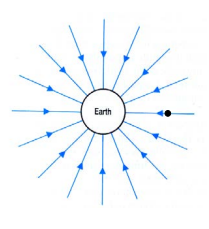
\includegraphics[scale=0.6]{assets/radialLines.png}
\end{center}\leavevmode
\\Near the surface of the Earth, where the Earth's curvature is negligible, the gravitational field lines are parallel and directed vertically downwards.
\begin{center}
    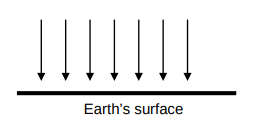
\includegraphics[scale=0.6]{assets/surfaceLInes.png}
\end{center}\leavevmode
\pagebreak
\section{Gravitational Field Strength}
\textbf{The gravitational field strength at a point in a gravitational field is defined as the gravitational force per unit mass acting on a small mass placed at that point.}
\\
\\In equation form:
\begin{equation}
    g=\frac{F}{m}
\end{equation}
\\
\\\textit{\small{*A test mass is an idealized model of an object whose physical properties are assumed to be completely negligible except for the property being studied, which is considered to be insufficient to alter the behaviour of the rest of the system.}}
\subsection{Gravitational Field Strength due to a Radial Field}
\begin{center}
    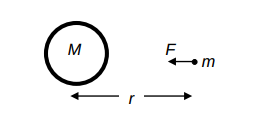
\includegraphics[scale=0.6]{assets/radialFieldGrav.png}
\end{center}\leavevmode Consider the Earth of mass $M$ and a point mass of $m$, placed at distance $r$ from the center of the Earth. The mass with experience a gravitational force towards the Earth.
We know the force acting on the mass is $F=\frac{GMm}{r^2}$. Therefore:
\\\begin{equation}
    g=\frac{F}{m}=\frac{(\frac{GMm}{r^2})}{m}=\frac{GM}{r^2}
\end{equation}

\subsection{Field Strength as Acceleration of Free Fall}
Consider a body of mass $m$ near the surface of the Earth falling towards the Earth as a result of gravitational force. The acceleration of $m$ is the acceleration due to free fall $a$.
\\
\\From Newtom's 2nd Law:
\begin{equation}
    \Sigma F=ma
\end{equation}

\begin{equation}
    \frac{GM_Em}{R_{E}^2}=ma
\end{equation}
\\Where $R_E$ is the radius of the Earth and $M_E$ is the mass of the Earth.
Therefore:
\begin{equation}
    a=\frac{GM_E}{R_E^2}
\end{equation}
\\We now have two ways of intrepreting $g$ at the Earth's surface:
\begin{enumerate}
    \item For any object, moving or at rest, the gravitational field strength is $9.81Nkg^{-1}$.
    \item For any object in free fall, the acceleration due to gravity is $9.81ms^{-2}$.
\end{enumerate}
\subsection*{Worked Example 2}
Assuming that the Earth is spherical with radius $6.4\times10^6$m and assuming $g=9.81Nkg^{-1}$ at the surface of the Earth, calculate the mass of the Earth. Hence, determine the average ensity of the Earth.
\\
\\\textbf{Solution}
\begin{equation}
    g=\frac{GM}{R^2}
\end{equation}
\begin{equation}
    M=\frac{gR^2}{G}
\end{equation}

\begin{equation}
    M=6.02\times10^{24}kg
\end{equation}
Using this value:
\begin{equation}
    \rho=\frac{M}{V}=\frac{M}{\frac{4}{3}\pi R^3}=\frac{3M}{4\pi R^3}=5.5\times10^3kgm^{-3}
\end{equation}
\\
\subsection*{Worked Example 3}
Assume the Earth to be a sphere of radius $r$ and mean density $\rho$. Show that the gravitational field strength of a point on its surface is $g=\frac{4}{3}G\rho\pi r$.
\\
\\\textbf{Solution}
\\Considering the sphere to behave as a point mass:
\begin{equation}
    g=\frac{GM}{R^2}=\frac{G\rho V}{r^2}
\end{equation}
Using the formula for the volume of a sphere, $V=\frac{4}{3}\pi r^3$:
\begin{equation}
    g=\frac{G\rho\frac{4}{3}\pi r^3}{r^2}=\frac{4}{3}G\rho\pi r
\end{equation}
\pagebreak
\section{Satellites in Orbits}
\subsection{Orbits around the Earth}
\begin{center}
    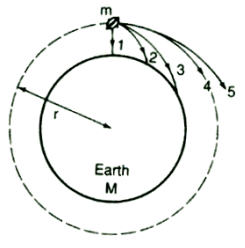
\includegraphics[scale=0.6]{assets/fallLines.png}
\end{center}\leavevmode
Consider an artificial satellite at some altitude from the Earth's surface. If it has not speed in the horizontal direction, it will fall towards the Earth along Path 1. 
If the horizontal speed is not sufficient, it will undertake Path 2 or 3. If the speed is too high, it will untake Path 5. However, with a specific speed, the satellite will undertake Path 4, or an orbit.
\\
\\For circular motion to take place, the gravitational force on the satellite provides the centripetal acceleration. Using the formula for angular velocity, $\omega=\frac{mv^2}{r}$:
\begin{equation}
    \frac{GM_Em}{r^2}=\frac{mv^2}{r}
\end{equation}
\begin{equation}
    v=\sqrt{\frac{GM_E}{r}}
\end{equation}
If the satellite is close to the Earth's surface, $r\simeq R_E$.
\subsection*{Worked Example 4}
A satellite of mass $m$ moves in a circular orbit about the Earth with a constant speed of $v$ and a height of $h=1000$km above the Earth's surface.
Determine the orbital speed of the satellite, given the radius of Earth is $6.4\times10^6$m and its mass is $6\times10^24$kg. Calculate, also, the period of revolution of the satellite.
\\
\\\textbf{Solution}
\begin{equation}
    \frac{GM_Em}{r^2}=\frac{mv^2}{r}
\end{equation}
\begin{equation}
    v=\sqrt{\frac{GM_E}{r}}
\end{equation}
The distance $r$ is the sum of the Earth's radius and the height of the satellite, meaning $r=R_E+h=7.4\times10^6$m. Therefore,
\begin{equation}
    v=\sqrt{\frac{GM_E}{r}}=\sqrt{\frac{(6.67\times10^{-11})(6\times10^{24})}{7.4\times10^6}}=7.35\times10^3ms^{-1}
\end{equation}
\begin{equation}
    v=r\omega=r(\frac{2\pi}{T})=7.4\times10^6(\frac{2\pi}{7.35\times10^3})=105min
\end{equation}
\subsection{Kepler's Third Law}
Consider a satellite of mass $m$, moving about the Earth of mass $M_E$ in a circular orbit. The satellite is orbiting about the Earth with an angular speed of $\omega$,
at radius $r$ from the center of the Earth, taking time $T$ to complete one orbit.
\begin{center}
    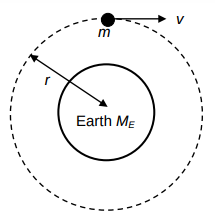
\includegraphics[scale=0.6]{assets/keplerDiagram2.png}
\end{center}\leavevmode
The gravitational force on the satellite provides the centripetal force for it to go along the circular orbit.
\begin{equation}
    \Sigma F_c=ma_c
\end{equation}
\begin{equation}
    \frac{GM_Em}{r^2}=mr\omega^2=mr(\frac{2\pi}{T})^2
\end{equation}
\begin{equation}
    T^2=(\frac{4\pi^2}{GM_E})r^3
\end{equation}
\\Since $\frac{4\pi^2}{GM_E}$ is a constant, $T^2 \propto r^3$. This is Kepler's Third Law: \textbf{For an orbiting body, the square of its period is proportional to the cube of its radius of orbit.} 
\subsection{Determining the Mass of Planets}
In 1798, Henry Cavendish made the first laboratory discovery of the value of $G$, the universal gravitational constant. Once this was done, it became possible to estimate the mass of the Earth.
By considering the motino of the moon and estimating the distance between them to be around $r=3.84\times10^8$m, we can show that the mass of the Earth $M_E$ is approximately $6\times10^24$.
\begin{center}
    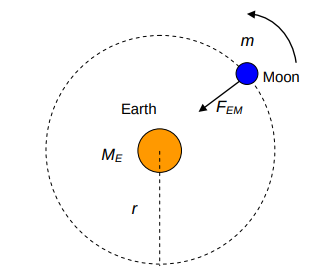
\includegraphics[scale=0.6]{assets/earthmoon.png}
\end{center}\leavevmode
Using the same methodology in the example above:
\begin{equation}
    \frac{GM_Em}{r^2}=mr(\frac{2\pi}{T})^2
\end{equation}
\begin{equation}
    M_E=\frac{4\pi^2r^3}{GT^2}
\end{equation}
Substituting for $G$, $r$ and since we know that the moon takes approximately one month ($T=2.36\times10^6$) to make one complete revolution around the Earth,
\\
\\$\Rightarrow M_E=6\times10^24$kg.
\\
\\Hence, we have found the mass of the Earth.
\pagebreak
\subsection{Geostationary Orbits}
An object in geostationary orbit will have the same orbital period as the mass it is orbiting. In other words, it has a fixed position in the sky with respect to a ground observer on the surface of the planet.
\\
\\For this to happen, the object must:
\begin{enumerate}
    \item Be directly above the Earth's equator. This is to ensure that the object rotates about the same axis as the Earth. If the object lies on other latitudes above the equator, its axis of rotation will not coincide with that of Earth's. As such, it's position would change and it will not be geostationary.
    \item Have an orbital period equal to the Earth's rotational period. This is to ensure that the object and the Earth will both rotate through the same angular displacement over the same time interval.
    \item Be orbiting from West to East.
\end{enumerate}
\begin{center}
    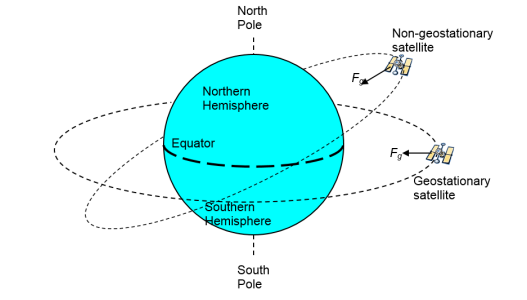
\includegraphics[scale=0.6]{assets/geostationary.png}
\end{center}\leavevmode
Geostationary satellites are useful as they allow antennas on Earth to constantly maintain a link with the satellite.
\subsection*{Worked Example 5}
Taking the radius of the Earth $R_E=6.4\times10^6$ and the mass of the Earth $M_E=6\times10^24$, determine the height of a geostationary orbiting satellite above the Earth's surface and its orbiting speed.
\\
\\\textbf{Solution}
\\For a geostationary orbit, $T=24$ hours $=24\times60\times60=86400$ seconds.
\begin{equation}
    \frac{GM_Em}{r^2}=mr(\frac{4\pi^2}{T^2})
\end{equation}
\begin{equation}
    M_E=(\frac{4\pi^2}{GM_E}) r^3
\end{equation}
\\
\begin{equation}
    r=\sqrt[3]{\frac{T^2GM_E}{4\pi^2}}=\sqrt[3]{\frac{(86400)^2(6.67\times10^{-11})(6\times10^{24})}{4\pi^2}}=4.23\times10^7
\end{equation}
\\
\begin{equation}
    h=r-R_E=(42.3-6.4)\times10^6=3.6\times10^7
\end{equation}
\\
\begin{equation}
    v=r\omega=4.23\times10^7\times\frac{2\pi}{86400}=3.1\times10^3ms^{-1}
\end{equation}
\subsection{Weightlessness in Orbit}
An astronaut orbiting the Earth is often said to be `weightless`. To understand why, let's try to weigh this astronaut.
\\
\\Consider the astronaut standing on a balance in space vehicle orbiting the Earth. Next, consider the space vehicle, astronaut and weighing balance as a single system.
\begin{center}
    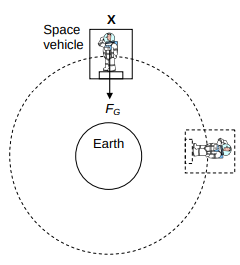
\includegraphics[scale=0.6]{assets/weighingAstronaut.png}
\end{center}\leavevmode
The only force acting on this system is the gravitational force due to the Earth's gravitational field, $F_G$. Since the vehicle is in a circular obit, $F_G$ provides the centripetal acceleration for the space vehicle to be in circular motion.
\\
\\Since $\Sigma F=M_{system}a$, we can use $M_{system}g=F$ to deduce that $a=g$. The vehicle, weighing machine and the astronaut all have the same acceleration $g$. Now consider the forces only acting on the astronaut. Suppose the astronaut is at position $X$ in the orbit.
\\
\\Again, since $\Sigma F=ma$, we can deduce that $mg-N=ma$, where $N$ is the force on the astronaut from the weighing balance.
However, since we've shown that $a=g$, the equation becomes $mg-N=mg$. 
\begin{center}
    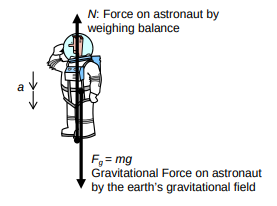
\includegraphics[scale=0.6]{assets/weighingAstronaut2.png}
\end{center}\leavevmode
Therefore, we see that the weighing balance does not exert a support force on the astronaut. By Newton's 3rd Law, the astronaut does not exert a force on its support. So, when the astronaut weighs himself, he sees that he is 'weightless.'
\pagebreak
\section{Gravitational Potential Energy}
\subsection{Gravitational Potential Energy $U$}
At infinity, the gravitational attraction of a spherical mass $M$ on a test mass $m$ is zero. We can therefore use this to deduce that the gravitational potential energy of mass $m$ at infinity is zero.
\\
\\Consider if mass $m$ is moved from infinity to a point, $A$, near the Earth by gravitational force $F_G$ alone.
The mass will gain kinetic energy as it is attracted by the field.
\\
\\In order to stop the mass from accelerating, an external agent is needed to apply an external force $F_{ext}$, acting in equal magnitude and opposite as $F_G$ so that the mass will move with a constant velocity towards $A$.
\begin{center}
    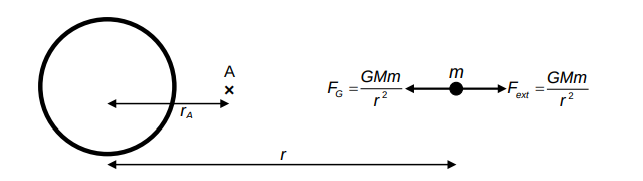
\includegraphics[scale=0.6]{assets/infinity.png}
\end{center}\leavevmode
\\
Since $F_G=\frac{GMm}{r}$, $F_{ext}$ must also be $\frac{GMm}{r}$. The work done by this external agent from infinity to point A is then $W_{ext}=\int_{\infty}^{F_A} F_{ext} \,dr =-\frac{GMm}{r_A}$, as work done is found by area under force-distance time graphs.
We deduced that there is no increase in kinetic energy. Therefore, all the work done by $F_{ext}$ is converted to gravitational potential energy. Therefore:
\begin{equation}
    U=-\frac{GMm}{r}
\end{equation}
\\
The gravitational potential energy of a mass at a point is defined to be \textbf{the work done by an external agent in bringing that mass from infinity to that point.}
\\
\\The gravitational potential energy will always be negative as gravitational fields are attractive - work is done \textit{on the object}, rather than done \textit{by the object}. 
\pagebreak
\subsection{Gravitational Potential}
The gravitational potential at a point in a field is defined to be the \textbf{work done per unit mass by an external agent in bringing a test mass from infinity to that point}. Note that gravitational potential and gravitational potential energy are two different things.
\\
\\As we deduced earlier, $U=-\frac{GMm}{r}$. This quantity is also equal to the work done by the external agent: $W_{ext}=-\frac{GMm}{r}$. Hence:
\begin{equation}
   \phi =\frac{W_{ext}}{m}=\frac{U}{m}=-\frac{GM}{r}
\end{equation}
\\
Where $\phi$ represents work done per unit mass.
\\
\\Let's summarise:
\begin{table}[h!]
    \centering
    \begin{tabular}{||c c||} 
     \hline
     Gravitational Potential Energy, $U$ & Gravitational Potential, $\phi$\\ [1ex] 
     \hline 
     It is a scalar value. & It is a scalar value.\\ [1ex]
     Magnitude is given by $U=W_{ext}$ & Magnitude is given by $\phi=\frac{W_{ext}}{m}$  \\[1ex]
     Radial magnitude is given by $U=-\frac{GMm}{r}$ &  Radial magnitude is given by $\phi=-\frac{GM}{r}$\\[1ex]
     Measured in $J$ & Measured in $Jkg^{-1}$\\[1ex]
     Dependent on both $M$ and $m$ & It is independent of $m$ and dependent on $M$.\\ [1ex] 
     \hline
    \end{tabular}
    \caption{Differences and Similarities.}\label{table:1}
\end{table}
\subsection*{Worked Example 6}
The diagram below shows two points $X$ and $Y$ at distances $R$ and $2R$ respectively from the center of the Earth. The gravitational potential at $X$ is $-8.0kJ kg^{-1}$.
\begin{center}
    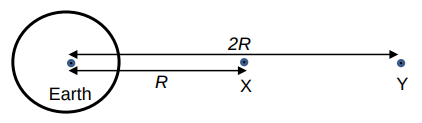
\includegraphics[scale=0.6]{assets/ex6.png}
\end{center}\leavevmode
Calculate the gain in gravitational potential energy of a $2$kg mass when it is moved from $X$ to $Y$.
\pagebreak
\\\textbf{Solution}
\begin{equation}
    \phi_x=-\frac{GM}{R}=-8kJkg^{-1}
\end{equation}
\begin{equation}
    \phi_y=-\frac{GM}{2R}=\frac{\phi_x}{2}=-4kJkg^{-1}
\end{equation}
\\
Therefore, the change in gravitational potential energy $\Delta U$ is:
\begin{equation}
    \Delta U=m\Delta\phi=2(\phi_y - \phi_x)=8kJ
\end{equation}
\\
\subsection*{Worked Example 7}
The figure below shows identical masses $m$ placed diametrically opposite and evenly spaced along the circumference of a circle with radius $r$. The point $X$ is the center of the circle.
\begin{center}
    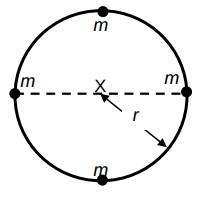
\includegraphics[scale=0.6]{assets/ex7.png}
\end{center}\leavevmode
\textbf{(a) (i)} Show that the potential at point $X$ is given by the expression $-\frac{4Gm}{r}$.
\begin{equation}
    \phi=(-\frac{Gm}{r})\times4=-\frac{4Gm}{r}
\end{equation}
\\
\textbf{(a) (ii)} State the work required to bring another identical mass from infinity to point $X$.
\begin{equation}
    W=\Delta U=(-\frac{4Gm^2}{r})-0=-\frac{4Gm^2}{r}
\end{equation}
\\
\textbf{(b)} State with reason the resultant gravitational field strength at point $X$.
\\
\\\textit{Since there are identical masses equidistant from $X$, the magnitude of their field strengths are also the same. The vector sum of their gravitational field strength is zero.}
\pagebreak
\subsection{Escape Velocity}
Suppose an object of mass $m$ is projected vertically upwards from the Earth's surface with an initial spped $v$. 
We can use energy considerations to find the minimum value of $v$ so that the object escapes the Earth's gravitational field.
\\
\\The gravitational potential energy of the object of mass $m$ at the surface of the Earth is given by:
\begin{equation}
    E_p=-\frac{GM_E m}{R_E}
\end{equation}
\\Assuming air resistance is negligible, the velocity of escape can be found by using the conservation of energy:
\begin{equation}
    (E_p+E_k)_{Earth}=(E_p+E_k)_{Infinity}
\end{equation}
Since $v_{esc}$ is the minimum speed to escape the field, we let $E_k$ and $E_p$ at infinity be equal to $0$.
\begin{equation}
    -\frac{GM_Em}{R_E}+\frac{1}{2}v^2_{esc}=0
\end{equation}
\\
\begin{equation}
    \frac{GM_Em}{R_E}=\frac{1}{2}v^2_{esc}
\end{equation}
\\
\begin{equation}
    v_{esc}=\sqrt{\frac{2GM_E}{R_E}}
\end{equation}
\subsection*{Worked Example 8}
For air at standard temperature and pressure, the velocity is $0.48kms^{-1}$. Taking the mass of the Earth to be $6\times10^24$kg and the radius of the Earth to be $6.4\times10^6$m, determine whether any hydrogen molecules will be lost from the atmosphere at a height of 100km.
\begin{equation}
    \frac{GM_E}{R_E+h}=\frac{1}{2}v^2_{esc}
\end{equation}
\\
\begin{equation}
    v_{esc}=\sqrt{\frac{2GM_E}{R_E+h}}
\end{equation}
\\
\begin{equation}
    v_{esc}=\sqrt{\frac{2(6.67\times10^{-11})(6\times10^{24})}{(6400+100)\times10^3}}=1.1\times10^4ms^{-1}
\end{equation}
\\
For air at standard temperature and pressure, the velocity of does not exceed the escape velocity. Therefore, hydrogen molecules would not be lost.
\pagebreak
\section{Equipotential and Potential Gradients}
A equipotential is a imaginary line where all points on it have constant potential. 
\begin{center}
    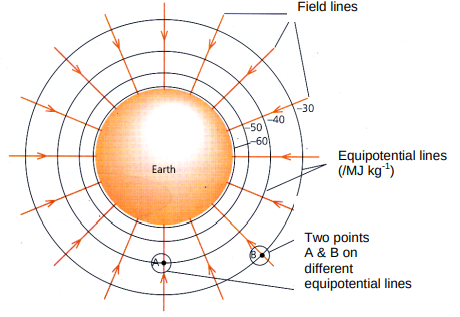
\includegraphics[scale=0.6]{assets/equipotentials.png}
\end{center}\leavevmode
Near the Earth's surface, equipotential lines are uniformly spaced. 1kg gains 9.81J of gravitational potential energy every 1m it is raised upwards.
\begin{center}
    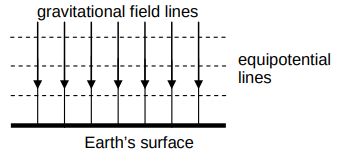
\includegraphics[scale=0.6]{assets/surfaceEquipotentials.png}
\end{center}\leavevmode
However, the farther away we get from the source of gravitational potential energy (in this case the center of the Earth), the equipotentials become non-uniform as field strength decreases.
Consider a test mass $m$ moved out by distance $\Delta r$ directly opposite gravitational force $F_G$.
\\
\\To move mass $m$ from $r_i$ to $r_f$ without gaining kinetic energy, work done by the external force must be equal to the gain in potential energy.
\begin{equation}
    F_{ext}=(r_f-r_i)=U_f-U_i
\end{equation}
\begin{equation}
    F_{ext}\Delta r=\Delta U
\end{equation}  
\begin{equation}
    F_{ext}=\frac{\Delta U}{\Delta r}
\end{equation}\leavevmode
\pagebreak
\\
\\When $\Delta$ r is small, $F_{ext}=\frac{dU}{dr}$. Since $F_{ext}=-F_g$, $F_g=-\frac{dU}{dr}$.
Also, since $F_g=mg$ and $dU=n\times d\phi$:
\begin{equation}
    mg=-m\frac{d\phi}{dr}
\end{equation}
\begin{equation}
    g=-\frac{d\phi}{dr}
\end{equation}
\section{Energy Conservation in the Motions of Planets and Satellites}
Consider a satellite of mass $m$ orbiting a planet of mass $M$ in a circular orbit. We know from previous sections that:
\begin{equation}
    E_p=-\frac{GM_E m}{r}
\end{equation}
\begin{equation}
    E_k=\frac{1}{2}mv^2
\end{equation}
\\
The gravitational force acting on the moon by the planet's gravitational field provides the centripetal force needed for circular motion.
When the total energy, which we know is $E_k+E_p$, is graphed with respect to distance, we see that:
\begin{center}
    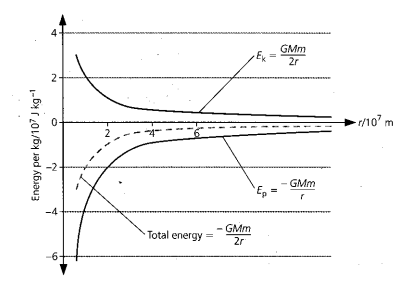
\includegraphics[scale=0.6]{assets/teGraph.png}
\end{center}\leavevmode
This particular graph applies for a satellite orbitting the Earth. The equations have been derived previously in these notes, however the derivation will be shown again, as follows:
\begin{equation}
    E_{total}=E_k+E_p
\end{equation}
\begin{equation}
    E_{total}=-\frac{GMm}{2r}-\frac{GMm}{r}
\end{equation}
\begin{equation}
    E_{total}=-\frac{GMm}{2r}
\end{equation}
\\
The total energy, $E_{tot}$, is always negative. Kinetic energy can never be negative, but as the seperation approaches infinity, it will also approach to zero. Potential energy will always be negative except for its zero value at infinity.
\\
\\The fact that $E_{tot}$ is negative denotes that the this satellite-Earth system is a bound system - there is gravitational force between them and satellite $m$ will never escape Earth's gravitational field.
\\
\\If the satellite were to be farther away from Earth, it would have greater (less negative) total energy. To escape from the center of force, the Earth, and still have $K_e$ at infinity, it would need positive total energy.
\\
\\A satellite orbiting the Earth will inevitably, albeit slowly, lose energy due to friction in the Earth's atmosphere. From the graphs, we see that as $E_{tot}$ decreases, $E_k$ increases and $E_p$ decreases. Therefore, as the satellite loses energy due to friction, it will gain speed and fall to a orbit of smaller radius. $E_p$ will decrease twice as much as $E_k$, hence there is a overall loss of energy.
\end{document}
